% % % % % % % % % % % % % % % % % Preamble for notes % % % % % % % % % % % % % % % % % % % % % % % %
\documentclass[12pt,oneside,a4paper]{article}


% % % % % Sprogpakker og Layout % % % % % % % % %
\usepackage[left=2.5cm,top=2.0cm,bottom=1.5cm, right=3.0cm]{geometry}
\usepackage{ulem}
\usepackage[danish,english]{babel}
\usepackage[utf8]{inputenc}
\linespread{1.3}       % simulerer Word 1.5 line spacing

% % % % % % % % % % Øvrige vigtige pakker % % % % %
\usepackage{graphicx}
\graphicspath{{./Figures/}}
\usepackage{amsmath}
\usepackage{amssymb}
\usepackage{url}
\usepackage{psfrag}
\usepackage{cancel}
\usepackage{booktabs}
\usepackage{pdfpages}
\usepackage{mathpazo}
\usepackage[section]{placeins}
\usepackage{caption}
\usepackage{wrapfig}
\usepackage{tocloft}
\usepackage{subcaption}
\usepackage{epstopdf}
\usepackage[separate-uncertainty = true]{siunitx}
\usepackage{fancyhdr}
%Muliggør 'flere figurer i én' Eksempel på anvendelse (indenfor figure-environment):
% \subfloat[undercaption 1]{\label{label 1}\includegraphics[bredde 1]{billede 1}}
% \subfloat[undercaption 2]{\label{label 2}\includegraphics[bredde 2]{billede 2}}
% \caption{overordnetcaption}
% \label{overordnet label}
\usepackage{lscape}
%Omdanner en del af dokumentet til landscape. Angives med \begin{landscape}
\usepackage{framed}
%Sætter en ramme om et område begrænset af \begin{framed} og \end{framed}.
%Allows footnotes
\usepackage{footnote}
\setlength{\parindent}{0cm}
\setlength{\parskip}{0.3cm}
% % % % % % COMMANDS % % % % % % % %

\numberwithin{equation}{section}
\begin{document}

\selectlanguage{english}
% % % % % % % % % % % % % % % % % % % % % % Forside % % % % % % % % % % % % % % % % % % % % % % % % %
\pagenumbering{roman}

\begin{center}
{\textsc {\LARGE \bf{Københavns Universitet \\[0.3cm]  Bachelorstudiet i fysik}}}\\[1.5cm]
{\textsc {\Large \bf Førsteårsprojekt 2017}}\\[0.8cm]
{\Large Projekt nummer: 2017-06}\\[1cm]

\rule{15cm}{0.01cm}\\[1cm]
{\LARGE\bf  Bouncing ball}\\ [0.5cm]
\rule{15cm}{0.01cm}\\[1cm]
\end{center}

\vfill
{\large Forfattere:}\\
{\large \hspace*{1cm} \makebox[6cm][l]{Andreas M. Faber}  \hspace{1cm} KU- ID: \makebox[2cm][l]{QZJ517} \\
{\large \hspace*{1cm} \makebox[6cm][l]{Benjamin T. Søgaard}   \hspace{1cm} KU- ID: \makebox[2cm][l]{MGX877} \\
{\large \hspace*{1cm} \makebox[6cm][l]{Joachim J. Kønigslieb}   \hspace{1cm} KU- ID: \makebox[2cm][l]{GWC666} \\

{\large Vejledere:}\\
{\large \hspace*{1cm} \makebox[6cm][l]{Jörg Helge Müller}  \hspace{1cm} Email: \makebox[2cm][l]{muller@nbi.ku.dk} \\

\vfill

{\large Rapporten omfatter {\bf 1} siders hovedtekst og {\bf 1} siders appendix.}

{\large Rapporten er indsendt som en pdf-fil den 17 marts 2017. }

\normalsize


% % % % % % % % % % % % % % % % % % % % % % Abstract  og Indholdsfortegnelse % % % % % % % % % % % % % % % % 
\newpage
\begin{abstract}
Kort resumé, gerne på både dansk og engelsk.
\end{abstract}

\newpage

\tableofcontents


% % % % % % % % % % % % % % % % % % % % % % Indhold % % % % % % % % % % % % % % % % % % % % % % % % %
\newpage
\pagenumbering{arabic}
\section{Introduction to chaos}
\label{chaos}
We will soon see that our experiment exhibits chaotic behavior. In physics, chaos is often described as a great dependance on initial conditions, meaning that two arbitrarily close initial conditions can make the system evolve into two states arbitrarily far apart (within some bounds). This is of course a rather loose definition, and it can therefor be useful to take a moment to examine a simpler chaotic system which has many of the same qualities our experiment has.

\subsection{The Logistic Map}

Consider the simple nonlinear recurrence relation


\begin{equation}
x_{n+1}=\lambda x_n (1-x_n)
\end{equation}


This is called the logistic map, and it has some interesting attributes. First of all, we will want to consider only cases where $0<x_0<1$ and $0<\lambda<4$, since outside these restrictions the series quickly diverges to $-\infty$. Within these restrictions, and if we at first limit ourselves to $\lambda<3$, no matter where on the interval $x_0$ starts, it seems to gravitate towards some value, dictated by $\lambda$, for increasing n. This value is called an attractor, and it is a common behaviour in nonlinear dynamical systems for there to be some point or region that attracts regions of initial conditions to it with increasing time or iterations.

\subsection{Cobweb diagrams}
The attractor can be visualized with a graphical algorithm with which the logistic map can also be easily iterated without use of a computer or calculator. First, we plot the functions $f(x)=\lambda x (1-x)$ and $g(x)=x$. Next, we choose an $x_0$. Now, we draw a vertical line from $x_0$ until it intersects $f(x)$. At the intersection we find the value of $x_1$ on the $y$-axis, since all we did was take our $x_0$ and plug it into the function $f(x)=\lambda x (1-x)$. To get $x_2$, we must now do what we just did with $x_0$, only for $x_1$. To this end we need to find $x_1$ on the $x$-axis instead of the $y$-axis. Therefor, we go horizontally to the graph for $g(x)=x$. The $x$- and $y$-coordinates of the intersection now both mark our value $x_1$, and we can vertically return to our graph of $f(x)$ to obtain $x_2$ on the $y$-axis, which we again convert to the $x$-axis by going to $g(x)$, and so on. Through many iterations and if sweeping for $0<x_0<1$ and $0<\lambda<3$, we see that for $n\to \infty$, $x_n$ tends towards these attractors. 



\begin{figure}
	\centering
	\caption{Independance of initial conditions in the cobweb diagram - $x_0$ has no effect on the value $x_n$ converges to}
	\label{cobweb}
	\begin{subfigure}{0.4\textwidth}
		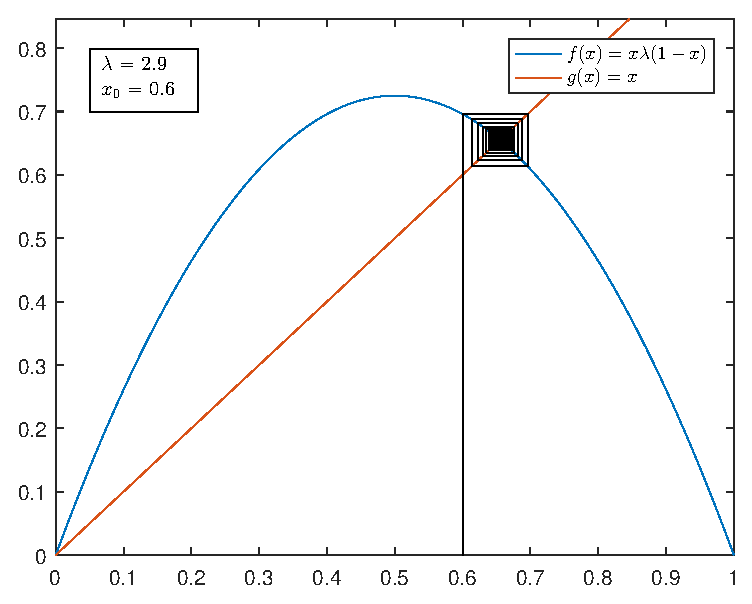
\includegraphics[width=\linewidth]{Figures/cobweb_x6_l29_iter50}
		\caption{Cobweb diagram with $x_0=0.6$ and $\lambda=2.9$}
		\label{}
	\end{subfigure}%
	\begin{subfigure}{.4\textwidth}
		\centering
		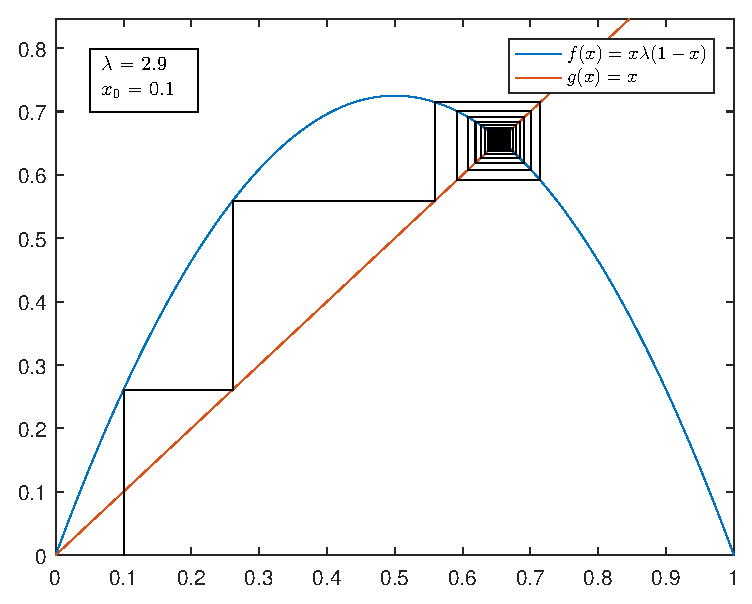
\includegraphics[width=\linewidth]{Figures/cobweb_x1_l29_iter50}
		\caption{Cobweb diagram with $x_0=0.1$ and $\lambda=2.9$}
		\label{}
	\end{subfigure}
\end{figure}




Examples of the first 50 or so iterations of this cobweb diagram can be seen for different $x_0$ and $\lambda$ on figure \ref{cobweb}, where it is clear that the attractor seems independant of the initial condition $x_0$, but dependant on $\lambda$. This dependance on $\lambda$ is very much worth investigating, since something remarkable happens if we permit $\lambda$ to be greater than 3.
\subsection{Bifurcation Diagrams}
For $\lambda$ slightly greater than 3, $x_n$ is not attracted to a single value, but rather starts bouncing between two distinct values as $n \rightarrow \infty$. For $\lambda$ even greater, $x_n$ will bounce between 4 values, then 8 and so on \footnote{cobweb diagrams of this behavior can be found in the appendix}. These sets of points are called an attractor. When the attractor splits and doubles the amount of points that attracts $x_n$, we call it a bifurcation, and it happens infinitely many times as we let $\lambda$ increase from 3 to 4. To try to get a better overview of this behavior, we can create what is called a bifurcation diagram. In this diagram, we sweep through different values of $\lambda$ and see where $x_n$ ends up. An example of this with $2<\lambda<4$ can be seen on figure \ref{bifurcation}.

\begin{figure}
	\centering
	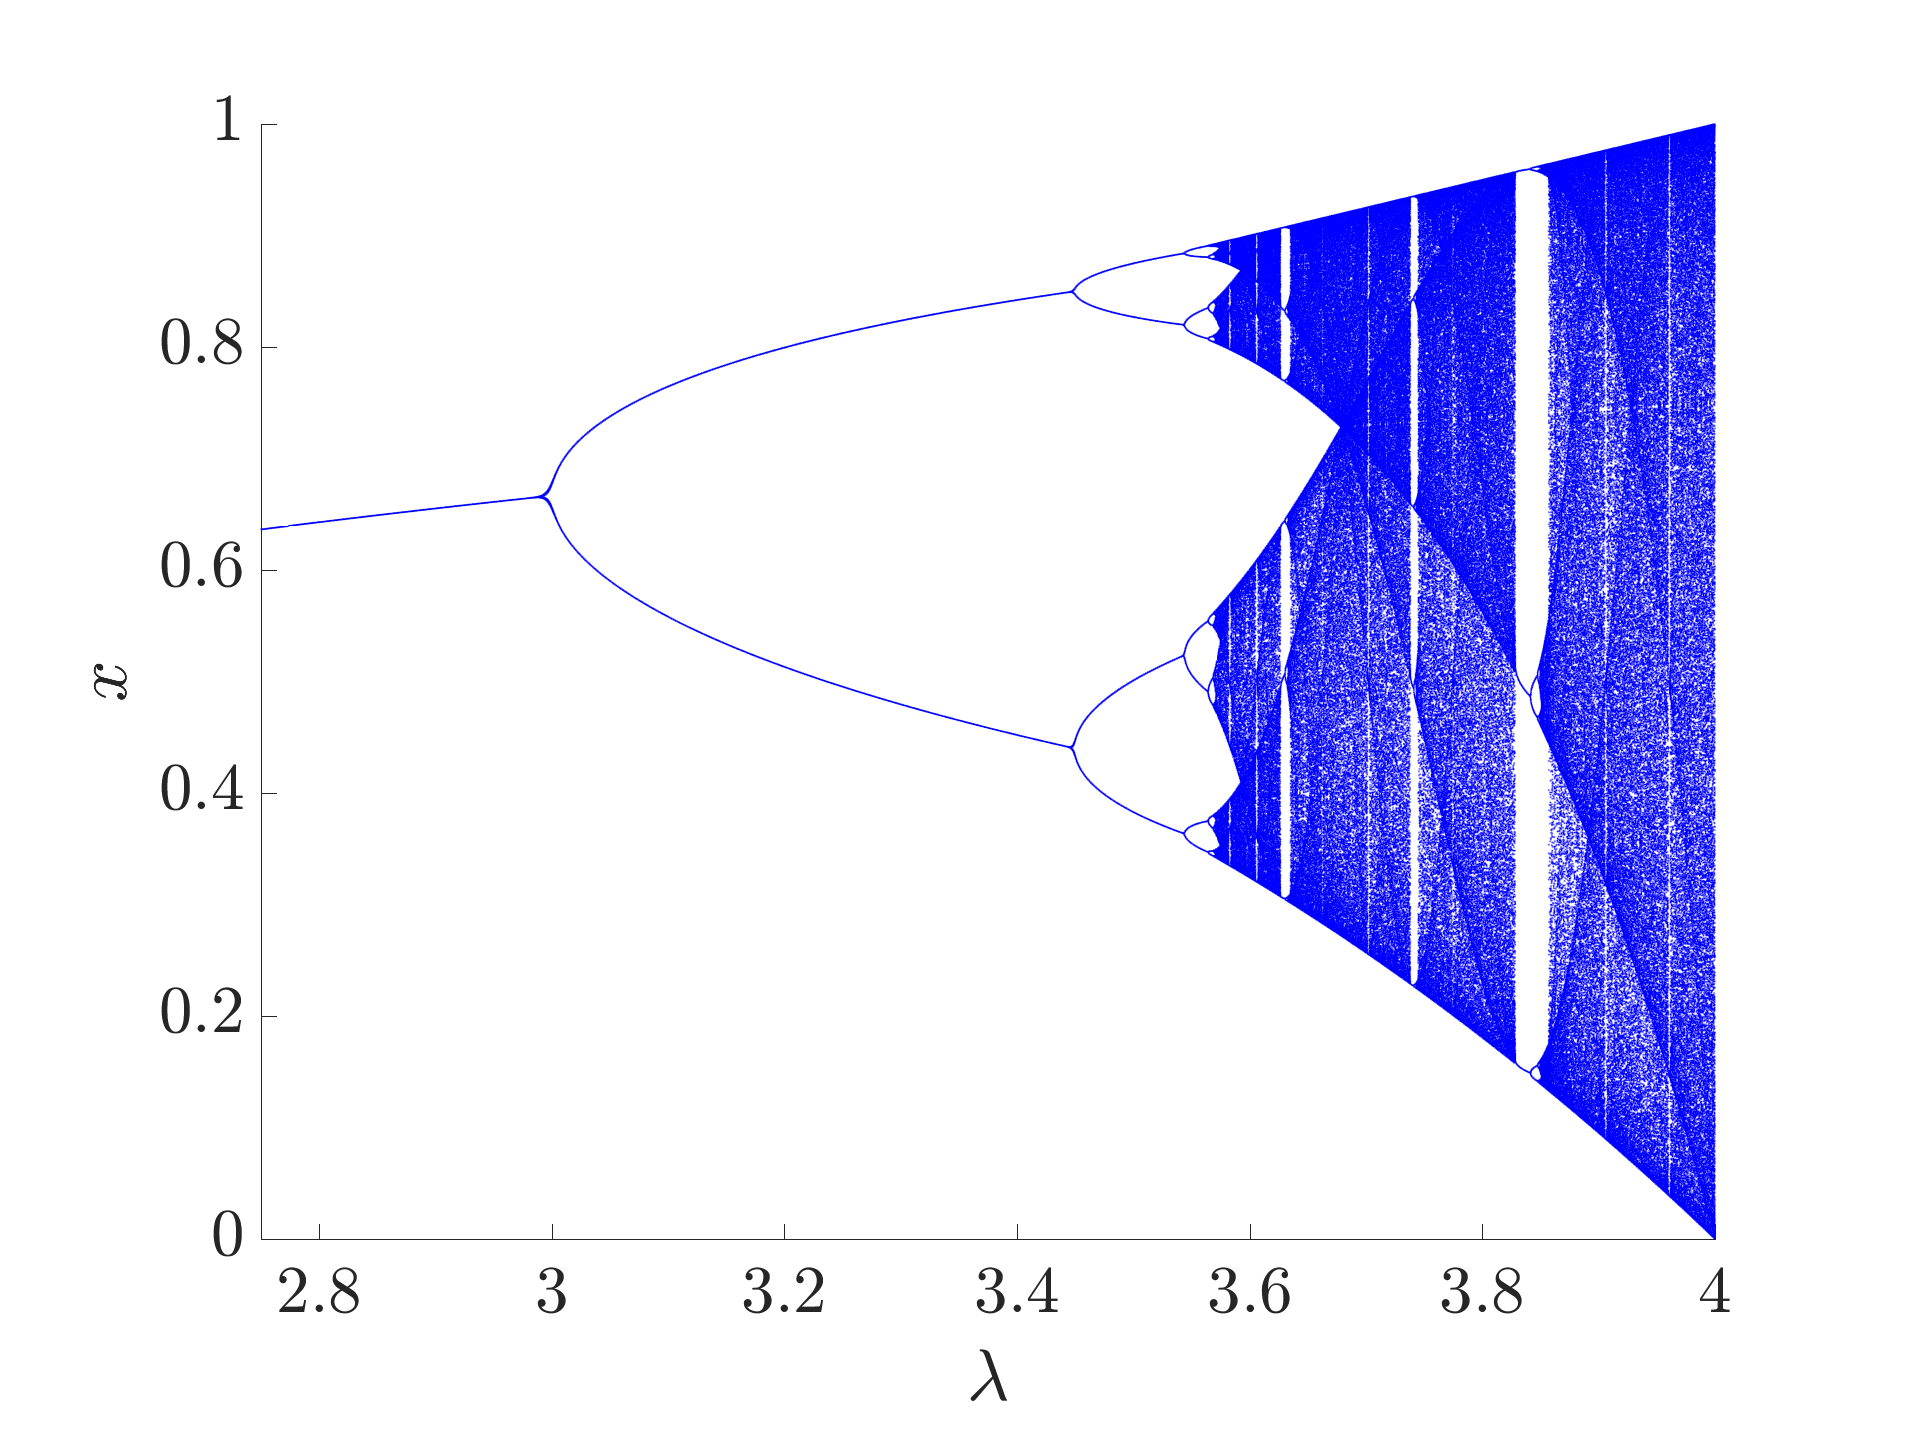
\includegraphics[width=0.8\linewidth]{Figures/Bifurcation}
	\caption{}
	\label{bifurcation}
\end{figure}


On the $x$-axis we have our different values of $\lambda$, and on the $y$-axis we plot the last 200 values of $x_n$ after 700 iterations. The key to understanding the bifurcation map is that we have 200 values of $x_n$ for each $\lambda$, which is of course what allows us to see the bifurcations. When we have a diagram like this, we can very clearly see the first couple of bifurcations, but at some point it seems like the plot just degenerates into chaos. The reason for this, is that the distance between each bifurcation decreases exponentially, so it very quickly becomes difficult to distinguish between 128 different values of $x_n$ that it cycles through, or pure chaos. However, as we continue to increase $\lambda$, we see islands where order reemerges from the chaos, and there briefly exists 3 attractors which then split to 6 and so on. It actually turns out that for any given number, there exists a region with that number somewhere in the diagram. How quickly after one another these bifurcations come can be approximated with something called Feigenbaums delta. Mitchell Feigenbaum found out, that as the number of bifurcations increase, the ratio between the distance between two consecutive bifurcations converges to a constant given by

\begin{equation}
\delta=\lim_{n \to \infty} \frac{\lambda_{n-2} - \lambda_{n-1}}{\lambda_{n-1}-\lambda_n} \approx 4.67
\end{equation}

Feigenbaum proved that this value converges to approximately 4.67, and that it does so rather quickly, which is important, because it means that it can be approximated rather reasonably with just the first 3 bifurcations. It also turns out that this constant holds (approximately) true for many other chaotic dynamical systems that display bifurcating nature, one of these systems being our bouncing ball. This is why we will give our estimate of Feigenbaums delta later, through both our simulation and experimental data.




\section{Model of the system}
\label{modelling}
\subsection{General model}
We will model our experiment as a 1-dimensional system that is we will not account for sideways motion. On figure \ref{bounces} two consecutive bounces can be seen where the later is bigger due to the plate  moving upwards at the time of impact.
\begin{figure}[h]
	\centering
	\includegraphics[width=0.6\textwidth]{Figures/bounceplot.eps}
	\caption{Plot of two bounces on the vibrating plate}
	\label{bounces}
\end{figure}
The $k^{\text{th}}$ bounce can be completely described by the time $t_k$ it left the plate and the velocity $v_k$ at that instance. Time and phases $\phi_k$ can be used interchangeably through the relationship $\phi=2\pi f t$.

To describe the system during a specific bounce we denote the distance of the ball above the plates rest position $y_b(t)$. Similarly we define $y_p(t)$ as the displacement of the vibrating  plate from it equilibrium. For a given frequency $f$, phase shift $\phi$ and amplitude $A$ the equation of motion for the plate is
\begin{equation}
	y_p(t)= A \cos(2\pi f t+ \phi)
	\label{platey}
\end{equation}
In air the ball is essentially a body in free fall, and since it is quite small and dense, the air resistance can be ignored. Thus the equation of motion for the ball $y_b(t)$ for the $k^\text{th}$ jump has the initial conditions $v_k$, $y_p(t_k)$ at time $t_k$, simply is
\begin{equation}
	y_{b,k}(t) = -\frac{g}{2}(t-t_k)^2+v_k(t-t_k)+y_p(t_k)
	\label{ybeq}
\end{equation}
For each jump we will denote the change of in initial $y$-coordinate\footnote{In general it is not possible to find $\Delta y_k$ analytically as it would require one to find the intersection between the graph of a parabola and a sine wave.} as $\Delta y_{k}=y_p(t_{k+1})-y_p(t_{k})$. Plugging that into (\ref{ybeq}) and solving for $t$ determines the fly time of each jump.
\begin{equation}
	\Delta t_{k} = t_{k+1}-t_{k} = \frac{v_{k}+\sqrt{v_k^2-2g\Delta y_k}}{g}
	\label{flytime}
\end{equation}
Further we can derive equation (\ref{ybeq}) finding the velocity of the ball thereby finding the final velocity for each jump $v_{k,f}$.
\begin{equation}
	v_{b,k}(t) = -g(t-t_k)+v_k \Rightarrow v_{k,f} = v_{b,k}(t_k+\Delta t_K) = -\sqrt{v_k^2-2g\Delta y_k}
\end{equation}
To model the impact between the ball and the plate we use a constant coefficient of restitution $C_r$ although more complex models have been suggested. For a plate at rest the velocity after the impact is proportional to the velocity before by $C_r$ such that $v_{up}=-C_r v_{down}$. For a moving plate we simplify transform into the coordinate system where the plate is at rest and then transform back. The velocity of the plate is easily obtain by deriving (\ref{platey}).
\begin{equation}
	v_p(t) = 2\pi f A \sin(2\pi f t+ \phi)
	\label{platev}
\end{equation}
Putting the two together yields the following relationship between the final velocity of the $k^{th}$ jump $v_{k,f}$ and the initial velocity of the next $v_{k+1}$.
\begin{align}
	v_{k+1} &= -C_r(v_{k,f}-v_p(t_k+\Delta t_k))+v_p(t_k+\Delta t_k) \nonumber \\
	&= C_r \sqrt{v_k^2-2g\Delta y_k}+2(C_r+1)\pi f A \sin(2\pi f (t_k+\Delta t_k)+ \phi) \label{impactv}
\end{align}
Equation (\ref{impactv}) looks quite complicated as it is for the most general case, but as we shall see in the next section it can be used together with a number of assumptions.

\subsection{1-Period stable}
If we consider the most simple stable state of our system, it is when the ball is bouncing with identical trajectories. A more formal way of stating it is that $\Delta t_k$ should be constant. By  (\ref{flytime}) this would further imply that the initial velocity $v_k$ is the same for every. For this to be true we must assume the phase at the impact also remain constant e.g. $\Delta y_k=0$. Which leads to the conclusion that the fly time must equal a whole number full period $\Delta t_k = \frac{n}{f}$ with $N\in \mathbb{N}$. Taking advantage of this fact together with (\ref{flytime}) yields the initial velocity for each jump
\begin{equation}
	\Delta t_k = \frac{n}{f} = \frac{2v_k}{g} \Rightarrow v_k = \frac{ng}{2f}
	\label{1perv}
\end{equation}
Denoting the phase of impact by $\theta$ we can simplify (\ref{impactv}).
\begin{equation}
	v_{k+1} = C_rv_k+2(C_r+1)\pi fA \sin(\theta)
\end{equation}
Substituting (\ref{1perv}) into the expression and solving for $\theta$ gives
\begin{align}
	\frac{ng}{2f} = C_r\frac{ng}{2f}+2(C_r+1)\pi fA \sin(\theta) \Rightarrow \sin(\theta) = \frac{ng}{4\pi Af^2 }\frac{C_r-1}{C_r+1}
	\label{1perstable}
\end{align}
The first thing to notice about (\ref{1perstable}) is that it does not have a solution for all parameter sets. That is not all settings can sustain a bouncing motion as they do not provide a sufficient amount of energy to balance the lose due to the impact. Since $\sin: \mathbb{R} \rightarrow [-1,1]$ we can determine when \eqref{1perstable} has a solution, the upper bound is ignored since the right hand side is clearly always negative.
\begin{align}
	-1 \le \frac{ng}{4\pi Af^2 }\frac{C_r-1}{C_r+1} \Rightarrow \sqrt{\frac{ng}{4\pi A}\frac{1-C_r}{C_r+1}} \le f
\end{align}
The above result is interesting in the sense that it is the lower frequency limit for a sustained bouncing motion. By deriving (\ref{platev}) again we can determine the minimum frequency for the ball to experience momentarily weightlessness is $f\ge\sqrt{\frac{g}{4\pi^2A}}$, the ratio between the two is
\begin{equation}
	r_f=\frac{\sqrt{\frac{g}{4\pi^2A}}}{\sqrt{\frac{ng}{4\pi A}\frac{1-C_r}{C_r+1}}} = \sqrt{\frac{1}{n\pi} \frac{1+C_r}{1-C_1}}
\end{equation}
We use a set-up with $C_r\approx 0.7$ and $n=1$ which gives $r_f\approx1.3$, that is the ball can get into a stable 1-period before the vibrating plate can start it by itself. It should be noted that the lower bound is greater in practice since the theoretical lower bound indicates when there is exactly enough energy in the system for a stable period. It is not however possible to provide the precise initial conditions to reached a stable period at that low frequencies. This is because of the effect just described where the plate does not oscillate fast enough for the ball to start bouncing. Also the this piece of theory suggest that a stable 1-period exists for all parameter sets high enough. In practice that is not true since the ball is much more likely to slip into a higher period at higher frequency. 

\section{The experiment}
\subsection{Schematic of the experimental setup}

\subsection{Characterization of the setup}
To perform the experiment we wish the parameters of the speaker membrane to independent of each other That is, amplitude should not depend of frequency, the 'sine-lyness' of the produced waveform should not depend of amplitude etc. This turned out to be not always the case. As the speaker is essentially a forced damped oscillator we observe some resonance behaviour, and our amplitude, in turn, was somewhat dependent on our frequency choice. For our chosen ball, the interesting frequency domain conceded with the natural frequency of the speaker. To mitigate this effect, we have measured characteristics of the speaker system in hopes of controlling \emph{both} apparent amplitude and frequency.  

Using an accelerometer attached to the side of the vibrating plate, we have measured the real amplitude of the system. We normalized the digital amplitude to range from 0 to 1, and measured the actual amplitude in the range \SI{14}{Hz} to \SI{30}{Hz} at digital 0.7. Then we used a cubic spline to interpolate the full range. Under the assumption that the actual amplitude is proportional to the digital amplitude. We created the following model of the amplitude as a function of frequency and digital amplitude, where $A_{0.7}(f)$ is the measured amplitudes.
\begin{equation}
	A(f,A_{d}) = A_{0.7}(f)\frac{A_{d}}{0.7} \Rightarrow A_d(f,A) = 0.7\frac{A}{A_{0.7}(f)}
	\label{ampl_model}
\end{equation}
As shown above we can use our model to predict the digital amplitude needed to match a required actual amplitude. A comparison of the uncorrected and corrected amplitude is show on figure \ref{frq_vs_ampl_plot}.
\begin{figure}[h]
	\centering
	\begin{subfigure}[t]{0.49\textwidth}
		\centering
		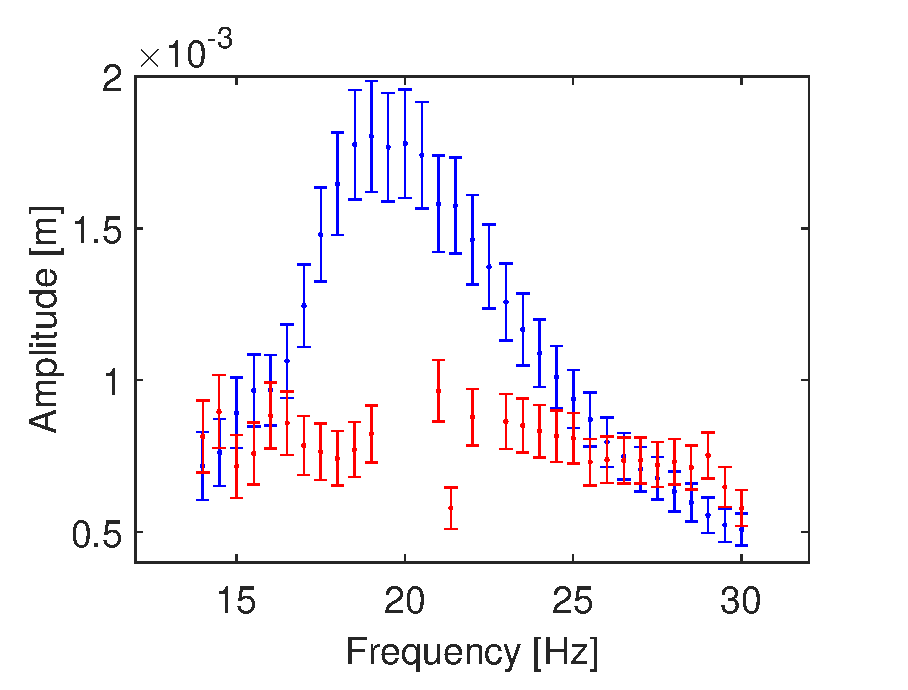
\includegraphics[width=\textwidth]{amplcorr.eps} 
		\caption{Frequency vs. amplitude, before and after corrections.}
		\label{frq_vs_ampl_plot}
	\end{subfigure}\hfill
	\begin{subfigure}[t]{0.49\textwidth}
		\centering
		\includegraphics[width=\textwidth]{surfplot}
		\caption{Surface plot of the amplitude model $A(f,A_{d})$ from \eqref{ampl_model}}
	\end{subfigure}
	\caption{Actual amplitude varies with the frequency for fixed digital frequency}
\end{figure}

 This model is not perfect, but limitations with our ability to measure one set frequency vs. amplitude for a large number of apparent amplitudes limits us to making assumptions about the system. We see our corrections is a significant improvement to blindly trusting the apparent values. The large error bars primarily comes from the conversion from acceleration to amplitude.

To get an idea of our baseline noise in measurements, we have collected a dataset comprised solely of noise. Taking the standard derivative will give us a measurement of the typical error. 

Seeing the plots of frequency vs amplitude, one might suspect the natural frequency of the system to be close to 20 Hz. To confirm this suspicion we have conducted two experiments. We also measured to real phase of the system and compared it to the apparent phase. The signal used to control the speaker will give us a reference $\pi\cdot N$ phase, which we have compared to the measured phase from accelerometer data. A plot of phase shift vs frequency looks like:
\begin{figure}[h]
	\centering
	\begin{subfigure}[t]{0.49\textwidth}
		
		\includegraphics[width=\textwidth]{pshiftplot.eps} 
		\caption{Phaseshift between the driven frequency and the real frequency.}
		\label{phaseshift_plot}
	\end{subfigure} \hfill 
	\begin{subfigure}[t]{0.49\textwidth}
		\centering
		\includegraphics[width=\textwidth]{ringout.eps}
		\caption{Ring-out of the speaker membrane after a sharp collision with fit $-2.13e^{-9.74t}\sin(127,6t+1.09)+2.96$}
		\label{ringout}
	\end{subfigure}
	\caption{Plots of various characteristics of the speaker}
\end{figure}
A derivation of the phase shifts dependency to driven frequency will be given in the appendix. This measurements corroborates our earlier suggestion of the natural frequency being right centred in the frequency domain of interest, suggesting the need for a correction model. 

\subsubsection{The coefficient of restitution}
On very important parameter in the setup is the coefficient of restitution $C_r$ which has already been described in the above. To measure it we used the fact the length of each jump on a plate at rest is proportional to the initial velocity. Since the jump the will be symmetric the initial and final velocity will be equal but with opposite signs. By equation (\ref{flytime}) and setting $\Delta y_k=0$ we can obtain the following ratio, which is exactly $C_r$.
\begin{equation}
	\frac{\Delta t_{k+1}}{\Delta t_{k}}= \frac{\frac{2v_{k+1}}{g}}{\frac{2v_{k}}{g}} = \frac{v_{k+1}}{v_k} = \frac{v_{k+1}}{v_{k,f}} = C_r
\end{equation}
As mentioned in section \ref{modelling} the coefficient of restitution is in fact not a constant as we assume but as function of impact velocity. Our measurement of the $C_r$ was therefore performed in by dropping the ball a few centimetres of the plate, which was at rest. This was done to emulate the conditions of the actual experiment while giving the ball enough energy to jump a few times. On average it bounced three times before coming to a rest. Through this small experiment we were able to determine $C_r= \num{0.659(5)}$ on the basis of 20 consecutive drops. 

\subsection{Collision between the ball and the plate}
It is obvious that the collision between the ball and the speaker will affect the waveform of the speaker. In the simple model, we assume that the speaker is ideal. That is, it will supply the needed impulse to change the momentum of the ball without being effected. By comparing the acceleration of the speaker with and without the ball, we can show the effect of bounces. 
\begin{figure}[h]
\centering
\includegraphics[width=\textwidth]{figure}
\caption{The waveform with and without the bouncing ball.}
\end{figure}
It seems that there is an effect, but that the acceleration of the speaker has returned to a normal sine waveform when the impacts occur. As the acceleration has taken a hit, we suggest that the velocity of the speaker will be lower than modelled. We also suggest that, as the speaker evidently isn't ideal, the speaker will not be able to provide the necessary impulse, and in turn, the ball will not have expected initial velocity out of the collision. 
\section{Numerical simulation}
As described in section \ref{modelling} it is not possible to solve the the systems equations of motion analytically in the general case as it require one to find the intersection between a parabola and a sine wave. In the numerical realm it is however possible to find a such intersection. The actual problem is to find where \eqref{platey} and \eqref{ybeq} are equal that is solving the following
\begin{equation}
	A \cos(2\pi f t+ \phi) = -\frac{g}{2}(t-t_k)^2+v_k(t-t_k)+y_p(t_k)
\end{equation}
As described this can easily be done numerically, and the initial velocity for the next jump follows from the equations derived in section \ref{modelling}. 

\subsection{Chaotic behaviour in the theoretical model}
The idea for the experiment originates from Tufillaro and Albano\cite{tufillaro}, who suggested that the bouncing ball behaves very much like the quadratic map described in section \ref{chaos}. We however discovered a wide range of chaotic behaviour even with a non-chaotic parameter set...
\subsection{Dependence on initial conditions}
We found trough numerical simulations that the systems behaviour strongly varies with different initial conditions. Most intriguingly we found that for some initial energies the system will fall into stable period-3 motion. This effect was very repeatedly demonstrated in the lab also. Trough numerical simulation we hoped to gain some insight into the connection between the initial velocities and the tendency to drop into period-3 motion as opposed to $2^n$-period motion. We have, for a fixed parameter set, plotted the difference between the times of the last jumps out of 1000 jumps, for varying values of initial velocity. 
\begin{figure}[h!]
\centering
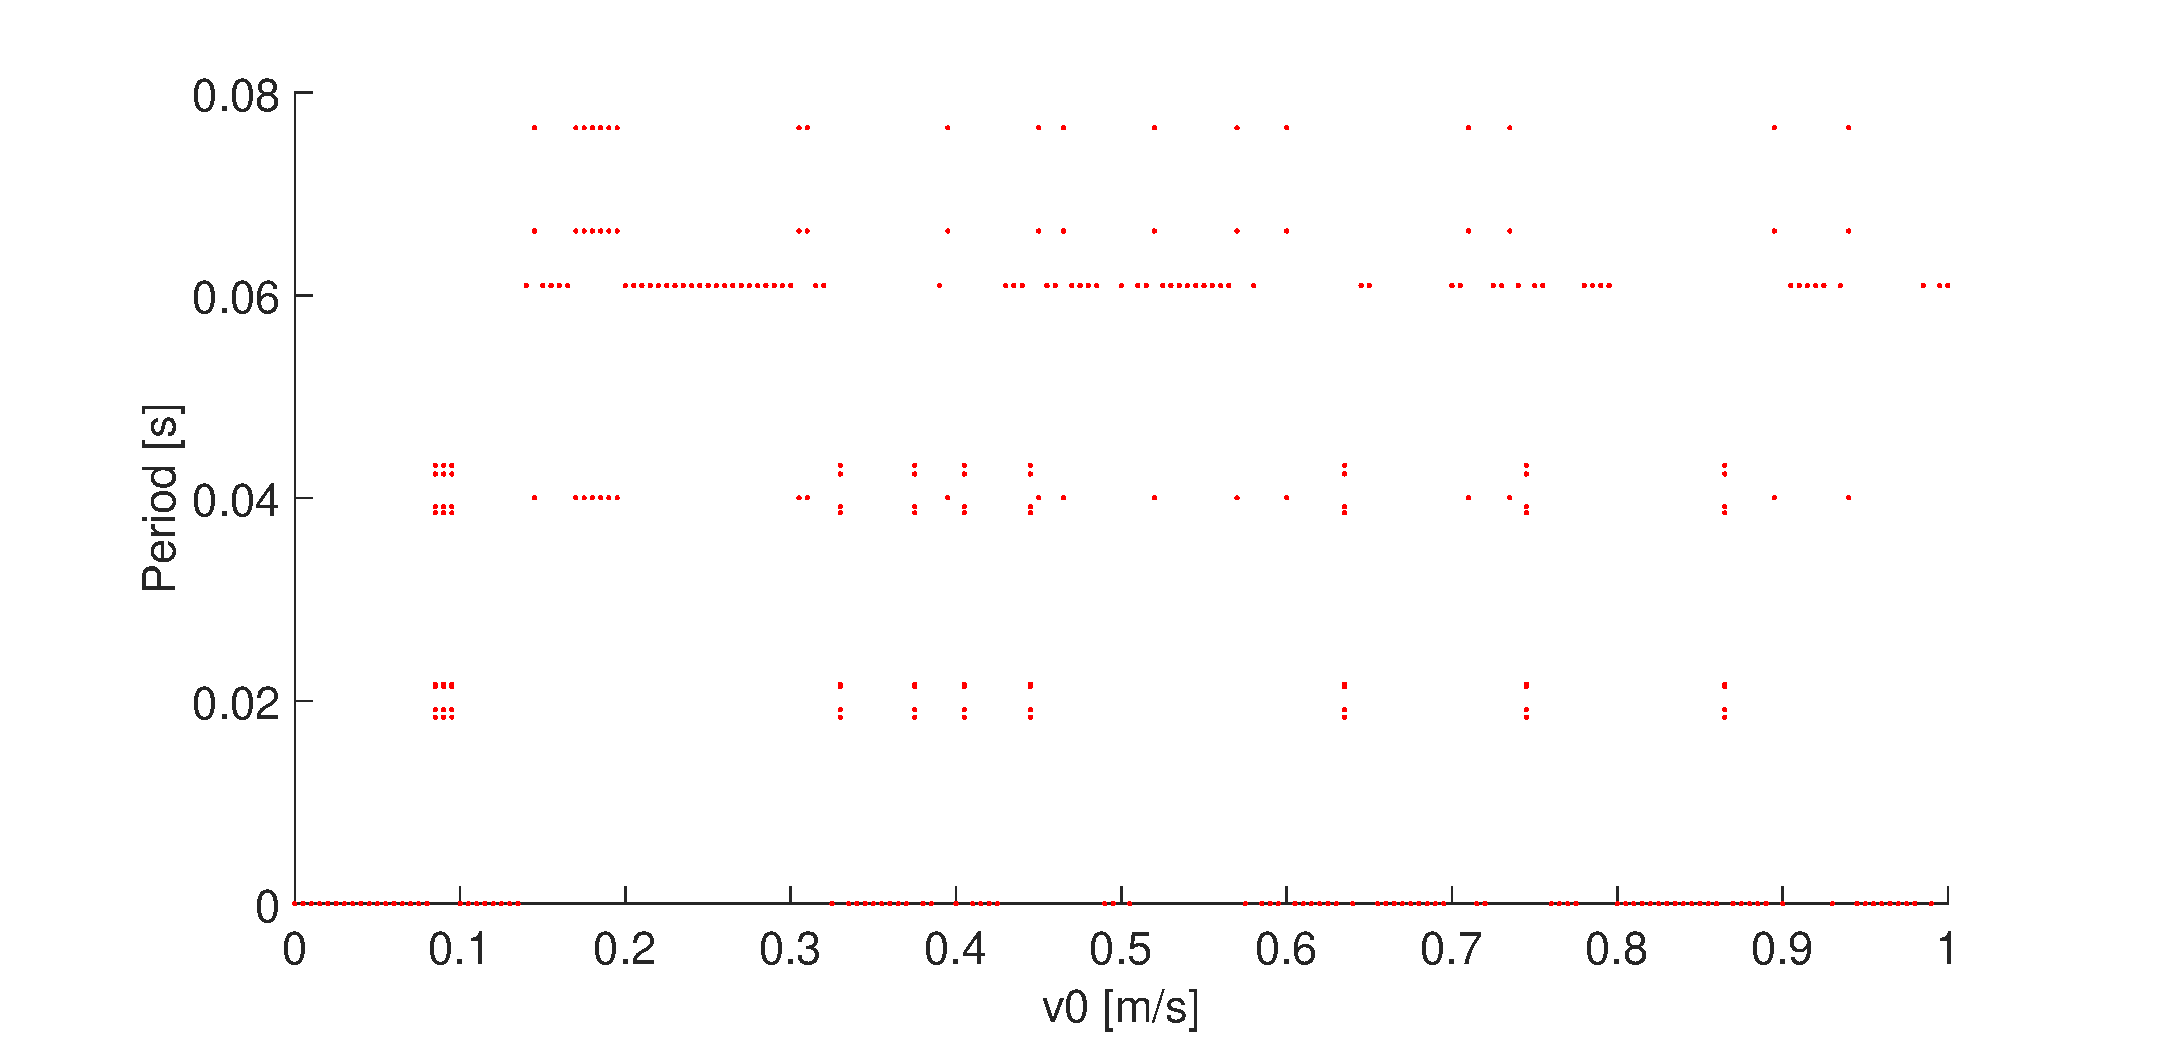
\includegraphics[width=0.95\textwidth]{vsweep.eps}
\caption{Stable solution depends strongly on initial velocity. The system plotted here is simulated with $C_r=0.66$, $f=\SI{16}{Hz}$, $A=\SI{1.1}{mm}$.}
\end{figure}
We cannot claim to identify any patterns in this, but we have found, that if we limit the initial velocity so that the ball won't skip a period, the simulations appear to be more stable. As mentioned this effect was also very prevalent in our experimental setup. Here we found that increasing the amplitude seemed to freeze out the 3-period mode, but for some initial conditions we could still arrive in the 3-period attractor. It should also be stressed that this period configuration was \emph{very} stable. 
\section{Data analysis}
\subsection{Comparison to simulated data}
\subsection{Feigenbaums $\delta$}
\section{Discussion and conclusions}
\newpage
\bibliographystyle{plain}
\bibliography{ref}

% % % % % % % % % % % % % % % % % % % % % % Appendix % % % % % % % % % % % % % % % % % % % % % % % % %
\newpage
\appendix
\section{Derivation of the equations of motion for a driven harmonic oscillator}
The equation of motion for a driven simple harmonic oscillator will be of the form:
\begin{align*}
my'' + by' + ky = F\sin(\omega t)\\
y'' + \frac{b}{m}y' + \frac{k}{m} y = F \sin(\omega t)
\end{align*}
We will then write the general solution as a sum of the particular and the homogeneous solutions:
\begin{align*}
y_g = y_{h} + y_p
\end{align*}
The homogeneous solution for the damped harmonic oscillator will go to zero with time. We claim it is only the particular solution that matters. To solve this, we will guess the solution to be of the form:
\begin{align*}
y_p = A \sin (\omega t) + B \cos(\omega t)
\end{align*}
We will perform the differentiation and plug into the equation to get:
\begin{align*}
&m\left(-A\omega^2\sin(\omega t) - B\omega^2\cos(\omega t)\right) + b\left(A\omega\cos(\omega t) - B\omega\sin(\omega t)\right) + k\left( A\sin(\omega t) + B\cos(\omega t) \right)\\
&=\sin(\omega t) \left( -mA\omega^2 -bB\omega + kA \right) + \cos(\omega t)\left(-mB\omega^2 + bA\omega + Bk\right)
\end{align*}
After collecting the coefficients, we can match the left side, with the right side:
\begin{align}
F &= -mA\omega^2 -bB\omega + Ak \label{lignA} \\ 
0 &= -mB\omega^2 + bA\omega + Bk \label{lignB}
\end{align}
We isolate an expression for $B$ in (\ref{lignB})
\begin{align*}
B &= \frac{-bA\omega}{-m\omega^2+k}
\end{align*}
Which we will proceed to plug into (\ref{lignA}), to obtain an expression for $A$:
\begin{align*}
A = \frac{F}{-m\omega^2+k+\frac{b^2\omega^2}{-m\omega^2+k}} = \frac{F\left(k-m\omega^2\right)}{\left(k-m\omega^2\right)^2+b^2\omega^2}
\end{align*} 
We can write $A$ and $B$ independently of each other:
\begin{align*}
B &= \frac{-bF\omega}{\left(k-m\omega^2\right)^2+b^2\omega^2}\\
A &=  \frac{F\left(k-m\omega^2\right)}{\left(k-m\omega^2\right)^2+b^2\omega^2}
\end{align*}
We would now like to express $y_p$ in the shape:
\begin{align*}
y_p = L \sin(\omega t + \phi)
\end{align*}
If we write the sine addition identity,
\begin{align*}
L sin(\omega t + \phi) = L\cos(\phi)\sin(\omega t) + L\sin(\phi)\cos(\omega t)
\end{align*}
We see, that our amplitude must obey,
\begin{align*}
A = L\cos(\phi)\\
B = L\sin(\phi)
\end{align*}
if we are to get our initial guess of
\begin{align*}
y_p = A \sin (\omega t) + B \cos(\omega t)
\end{align*}
The phase shift will then be:
\begin{align*}
\frac{B}{A} &= \frac{L\sin(\phi)}{L\cos(\phi)} = \tan(\phi)\\
\phi &= \arctan\left(\frac{B}{A}\right)\\
\phi &= \arctan\left( \frac{-bF\omega}{\left(k-m\omega^2\right)^2+b^2\omega^2} \cdot \frac{\left(k-m\omega^2\right)^2+b^2\omega^2}{F\left(k-m\omega^2\right)} \right)\\
\phi &= \arctan\left( \frac{b\omega}{m\omega^2-k} \right)
\end{align*}
\end{document}
